\begin{figure*}[ht]
    \centering
    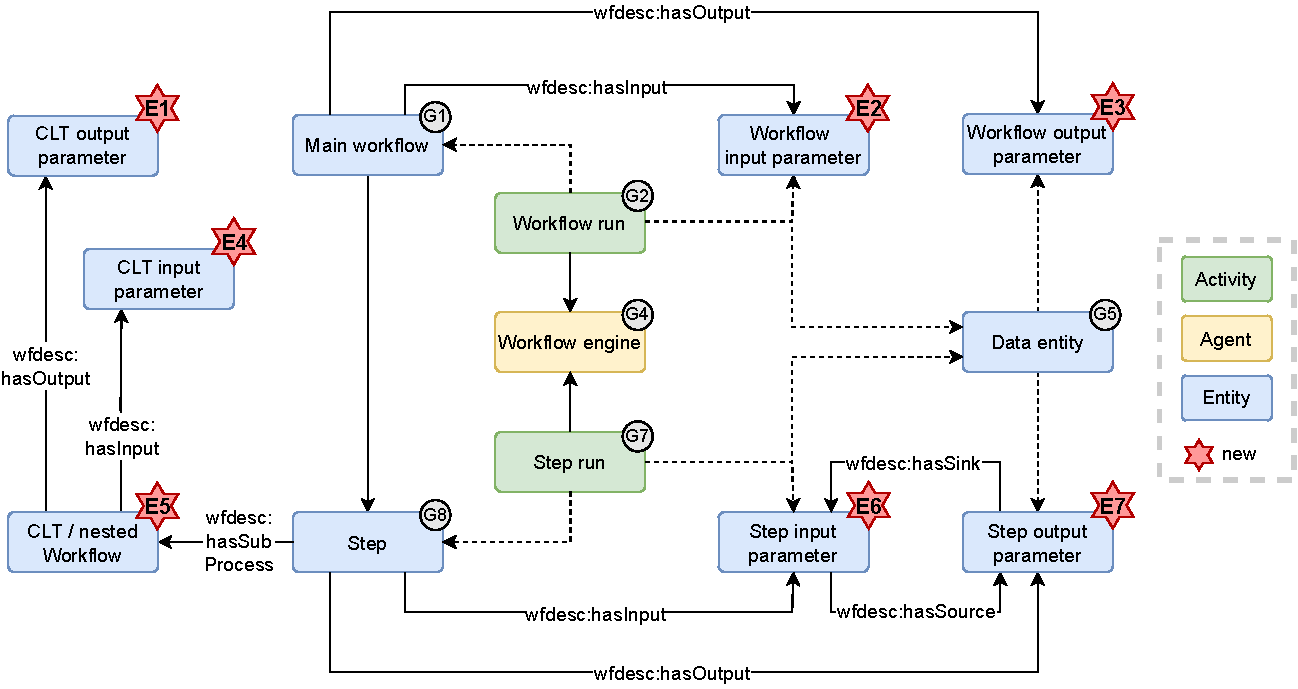
\includegraphics[width=0.99\textwidth]{rdf_extension/CWLProv_graph_extended.pdf}
    \caption{The RDF provenance graph, now extended with \emph{CommandLineTools} and parameter entities. Red stars mark nodes which are part of the design extension. Parameters are linked to their \emph{Workflow}, \emph{CommandLineTool} or step via \emph{wfdesc:hasInput} and \emph{wfdesc:hasOutput}. Node G5 represents both input and output data entities. The data flow between steps is represented via \emph{wfdesc:hasSink} and \emph{wfdesc:hasSource}. Steps are linked to their underlying tools via \emph{wfdesc:hasSubProcess}.}
    \label{fig:cwlprov_graph_new}
\end{figure*}

